%!TEX root = paper.tex

Rather than looking at an explicit representation of lines in the plane, we can gain much more insight from looking at a parametric representation. To simplify our analysis, we will choose our time parameter such that v collisions occur every $\Delta t = 1$ and h collisions occur every $\Delta t = m$. The equation for a line $y(x) = m \, x + b$ is equivalent to the following parametric system

\begin{align}\label{eq:parametric-line}
	x(t)& = \frac{1}{m} \, t + x_0\\
	y(t)& = t
\end{align}

Now v and h collisions in the 2-dimensional plane can be projected onto the 1-dimensional $t$ axis.

\begin{figure}[H]
  \begin{center}
    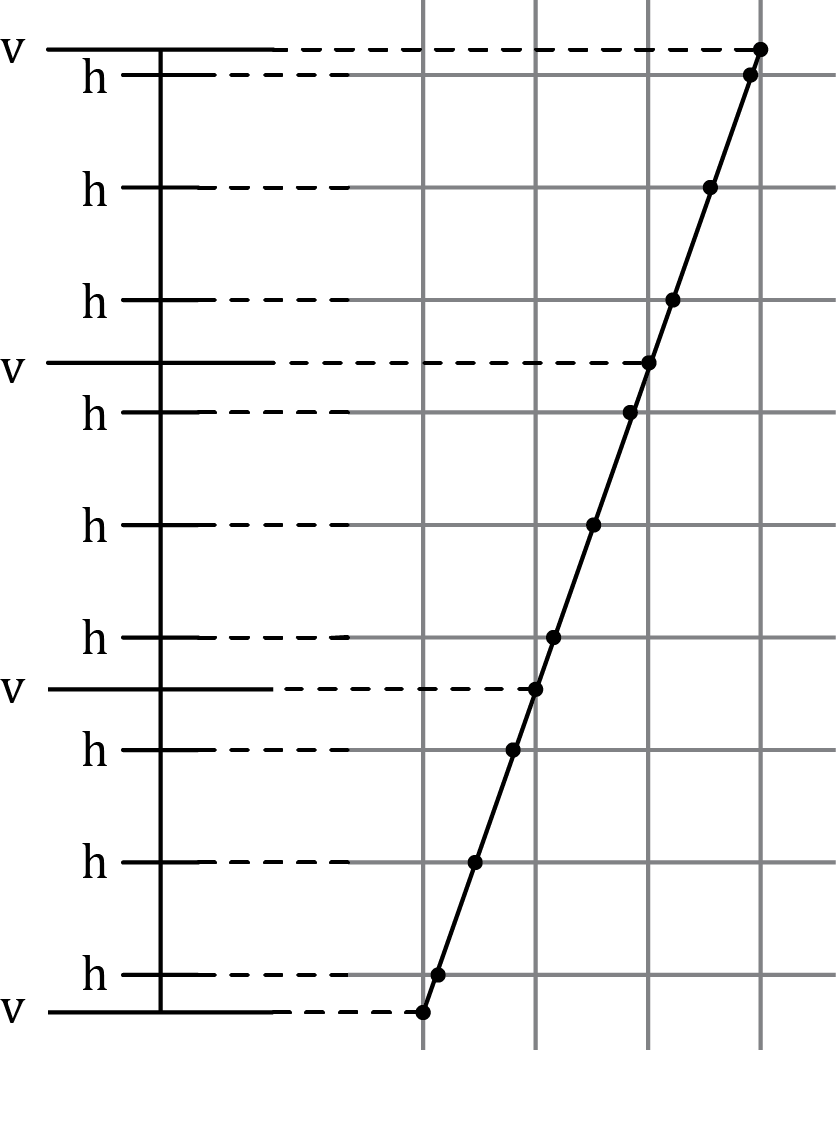
\includegraphics[keepaspectratio, width=4in]{1d_mapping_1.png}
  \end{center}
  \vspace{-.2in} % corrects bad spacing
  \caption{\label{fig:1d-projection} Projecting onto the parametric representation.}
\end{figure}

For the sake of space, we will rotate the $t$ axis so that it is horizontal.

\begin{figure}[H]
  \begin{center}
    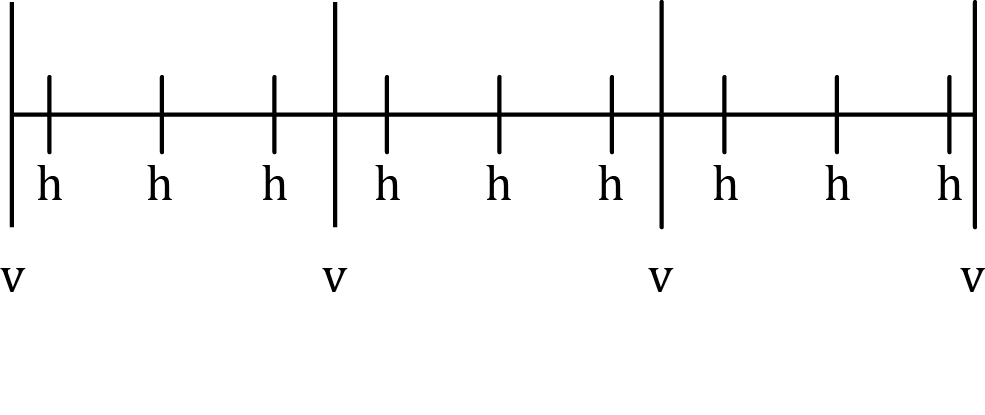
\includegraphics[keepaspectratio, width=4in]{1d_mapping_2.png}
  \end{center}
  \vspace{-.2in} % corrects bad spacing
  \caption{\label{fig:1d-problem} Projecting onto the parametric representation.}
\end{figure}

% -----------------------------------------------------------------------------

\begin{lemma}\label{lem:interval-ticks}
	The number of real numbers spaced at regular intervals $l_2$ inside an interval of length $l_1$ is in $\cbracket{\floor{\frac{l_1}{l_2}}, \ceil{\frac{l_1}{l_2}}}$.
\end{lemma}

\begin{proof}
	Let $A \subset \Z$ represent the set of all possible numbers of real numbers spaced at regular intervals $l_2$ inside an interval of length $l_1$. Given some $a \in A$, let $b \in \R$ be defined such that the following holds

	\begin{equation}\label{eq:interval-ticks}
		l_1 = (a - 1) l_2 + b
	\end{equation}

	We know that $(a - 1) l_2 \le l_1$, so $b \ge 0$. Also, $b < 2$ because otherwise, there must be more than $a$ real numbers inside the interval, contradicting our original assumption.

	Rearranging Equation \ref{eq:interval-ticks}, we get

	\begin{equation}
		a = \frac{l_1}{l_2} + 1 - \frac{b}{l_2}
	\end{equation}

	Which leads directly to

	\begin{equation}
		a \in \cbracket{\floor{\frac{l_1}{l_2}}, \ceil{\frac{l_1}{l_2}}}
	\end{equation}
\end{proof}

% -----------------------------------------------------------------------------

\begin{lemma}\label{lem:h-extension}
	A finite sequence $\alpha$ is a valid collision sequence iff there exists at least one valid collision sequence containing $\alpha$ that starts and ends with an h.
\end{lemma}

\begin{proof}
	TODO: can extend any collision sequence to any length. 
\end{proof}

% -----------------------------------------------------------------------------

Because of Lemma \ref{lem:h-extension}, without loss of generality we can confine ourselves to only look at collision sequences that start and end with an h.

\begin{definition}
	Given a collision sequence $\alpha$, define a sequence $\beta^{(0)}$ where each element $\beta^{(0)}_i$ is the number of h collisions between the i\textsuperscript{th} and (i+1)\textsuperscript{th} v in $\alpha$.
\end{definition}

The $\beta^{(0)}$ sequence is much simpler to think of geometrically. Looking at Figure \ref{fig:beta-sequence}, $\beta^{(0)}_i$ represents the number of h tick marks in between each v tick mark.

\begin{figure}[H]
  \begin{center}
    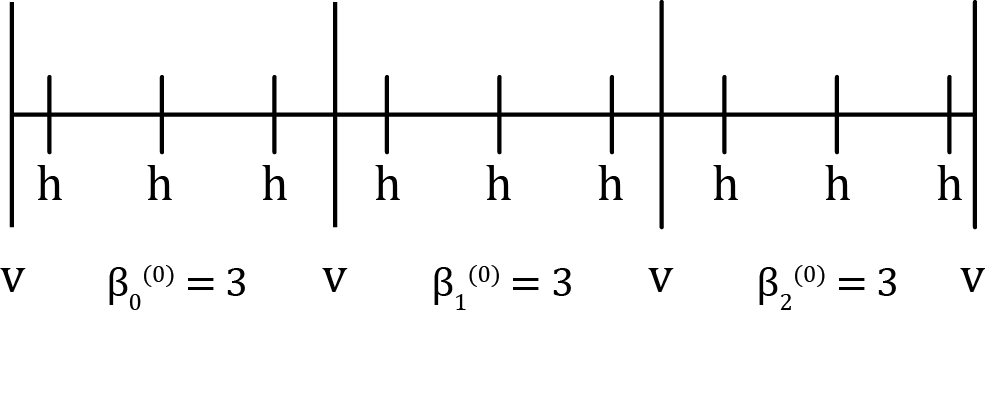
\includegraphics[keepaspectratio, width=4in]{1d_mapping_3.png}
  \end{center}
  \vspace{-.2in} % corrects bad spacing
  \caption{\label{fig:beta-sequence} The $\beta^{(0)}$ sequence.}
\end{figure}

\begin{definition}
	Given a valid collision sequence, define the sequence $\beta^{(j)}$ where each element $\beta^{(j)}_i$ is 1 more than the number of occurrences of $\beta^{(j-1)}_{max}$ between the i\textsuperscript{th} and (i+1)\textsuperscript{th} occurrence of $\beta^{(j-1)}_{min}$ in the $\beta^{(j-1)}$ sequence.

	If, for some $j_f$, the length of $\beta^{(j_f-1)}$ is 1, then $\beta^{(j_f-1)}$ is the terminating ``meta'' sequence, and all subsequent $\beta^{(j)}$ for $j \ge j_f$ are undefined.
\end{definition}

An example $\beta^{(j)}$ sequence is plotted in Figure \ref{fig:beta-sequence-j}.

\begin{figure}[H]
  \begin{center}
    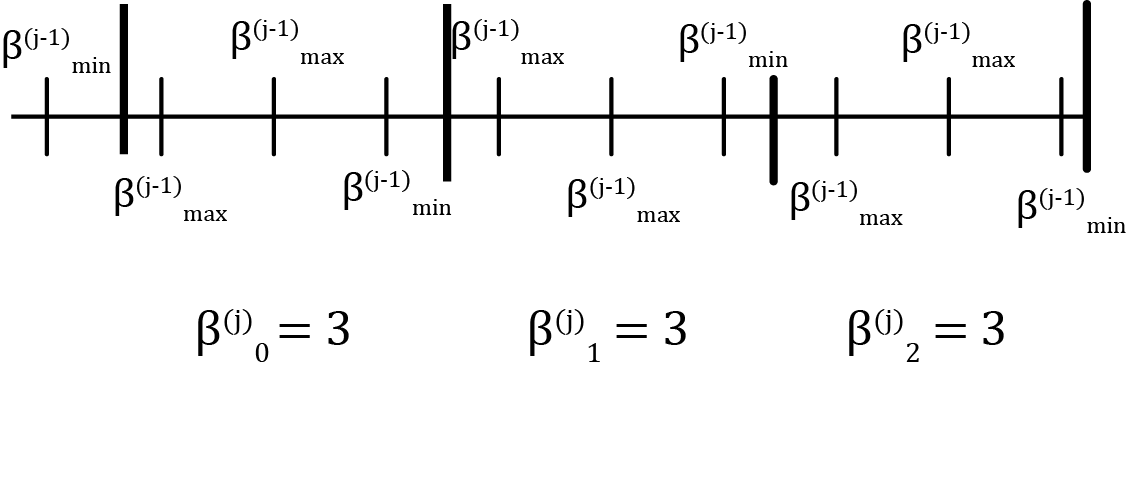
\includegraphics[keepaspectratio, width=4in]{1d_mapping_5.png}
  \end{center}
  \vspace{-.2in} % corrects bad spacing
  \caption{\label{fig:beta-sequence-j} The $\beta^{(j)}$ sequence.}
\end{figure}

Now we can derive a very useful sequence that we will call $a$. We start with $a_0 \coloneqq m, a_1 \coloneqq 1$. These two values represent the two intervals sizes in our parametric representation.

\begin{figure}[H]
  \begin{center}
    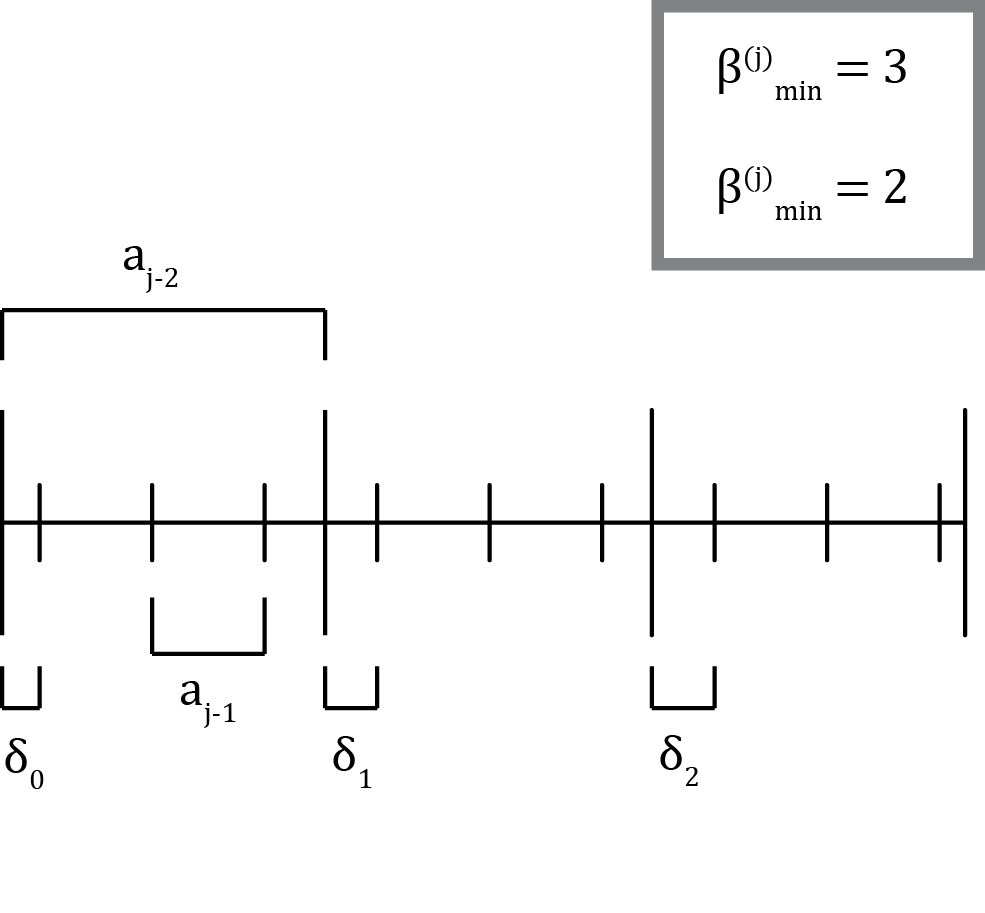
\includegraphics[keepaspectratio, width=4in]{1d_mapping_4.png}
  \end{center}
  \vspace{-.2in} % corrects bad spacing
  \caption{\label{fig:a-sequence} The $\beta^{(i)}$ sequence.}
\end{figure}

From Lemma \ref{lem:interval-ticks}, we know that $\beta^{(0)}_{max} = \ceil{\frac{m}{1}}$. 

\begin{align}\label{delta_beta}
	\delta^{(0)}_i \coloneqq \begin{cases}
		x_0 \qquad &\text{for} \quad i = 0\\
		i (\beta^{(0)}_{max} * 1 - m) + x_0 \qquad &\text{for} i \ge 1
	\end{cases}
\end{align}

We can notice that

\begin{align}\label{eq:beta_i}
	\beta^{(0)}_i = \floor{\delta^{(0)}_i} + \beta^{(0)}_{max} - \floor{\delta^{(0)}_{i+1}}
\end{align}

Thus if we plot the values of $\delta^{(0)}$ we can see an interesting pattern of the $\beta$

The rest of $a$ will be defined inductively. For $2 \le j < j_f$, assume that $a_{j-1}, a_{j-2}$.

\begin{align}\label{delta_beta}
	\delta^{(j)}_i \coloneqq \begin{cases}
		x_0 \qquad &\text{for} \quad i = 0\\
		i (\beta^{(j)}_{max} * 1 - m) + x_0 \qquad &\text{for} i \ge 1
	\end{cases}
\end{align}

The number of tick marks in each interval is $\beta^{(0)}$
Now from \ref{lem:interval-ticks}, we know that 

\begin{align}
	\gamma = \ceil{\frac{a_{j-1}}{a_{j-2}}}
\end{align}

$\gamma$ represents the smallest integer number of intervals of length $a_{j-1}$ that can cover an interval of length $a_{j-2}$. Thus at most $\gamma$ tick marks with spacing $a_{j-1}$ can fit inside an interval of length $a_{j-2}$. 

This sequence is written concisely in the following definition

\begin{definition}
	Define the sequence $a$

	\begin{equation}
		a_j \coloneqq \begin{cases}
			m \qquad &\text{for} \quad j = 0\\
			1 \qquad &\text{for} \quad j = 1\\
			\beta^{(j-2)}_{max} a_{j-1} - a_{j-2} \qquad &\text{for} \quad 2 \le j < j_f
		\end{cases}
	\end{equation}

\end{definition}

From now on we will only consider collision sequences, where each non-terminal $\beta^{(j)}$ starts and ends with $\beta^{(j)}_{min}$.

% -----------------------------------------------------------------------------

\begin{theorem}\label{thm:beta_i}
	A collision sequence is valid iff the following is true for all $j$

	\begin{equation}
		\beta^{(j)}_i \in \cbracket{\floor{\frac{a_{j-2}}{a_{j-1}}}, \ceil{\frac{a_{j-2}}{a_{j-1}}}}
	\end{equation}
\end{theorem}

\begin{proof}
	This was already proved above, we are just stating it again.
\end{proof}

% -----------------------------------------------------------------------------

\begin{theorem}
	For every valid collision sequence, $\lim_{n \to \infty} a = 0$
\end{theorem}

\begin{proof}
	From the definition of $a_j$

	\begin{align}\label{eq:a-def-2}
		a_j& = \beta^{(j-2)}_{max} \, a_{j-1} - a_{j-2}\\
		& =  \ceil{\frac{a_{j-2}}{a_{j-1}}} a_{j-1} - a_{j-2}
	\end{align}

	Now from the definition of the ceiling function, we know that

	\begin{equation}
		0 \le \ceil{\frac{a_{j-2}}{a_{j-1}}} - \frac{a_{j-2}}{a_{j-1}} < 1
	\end{equation}

	Rearranging, we get

	\begin{equation}
		0 \le \ceil{\frac{a_{j-2}}{a_{j-1}}} a_{j-1} - a_{j-2} < a_{j-1}
	\end{equation}

	Combining the above equation with Equation \ref{eq:a-def-2}, we get

	\begin{equation}
		0 \le a_j < a_{j-1}
	\end{equation}

	Thus $a$ is strictly decreasing and bounded below by 0, so $\lim_{n \to \infty} a_n = 0$.
\end{proof}